% =============================================================================
% CAPITULO 2: MARCO TEORICO
% =============================================================================

\chapter{Marco Teorico}
\label{ch:marco_teorico}

Este capitulo presenta los fundamentos teoricos necesarios para comprender la arquitectura y metodologia desarrollada en este trabajo. Se abordan los conceptos de redes neuronales convolucionales, arquitecturas modernas, mecanismos de atencion, funciones de perdida especializadas y tecnicas de preprocesamiento de imagenes medicas.

% -----------------------------------------------------------------------------
\section{Redes Neuronales Artificiales}
\label{sec:redes_neuronales}
% -----------------------------------------------------------------------------

\subsection{Perceptron y Redes Multicapa}

Las redes neuronales artificiales estan inspiradas en el funcionamiento del cerebro biologico. La unidad basica es el \textit{perceptron}, introducido por Rosenblatt en 1958 \cite{rosenblatt1958perceptron}, que computa una suma ponderada de sus entradas y aplica una funcion de activacion:

\begin{equation}
    y = \phi\left(\sum_{i=1}^{n} w_i x_i + b\right) = \phi(\vec{w}^T \vec{x} + b)
    \label{eq:perceptron}
\end{equation}

donde $\vec{x} \in \R^n$ es el vector de entrada, $\vec{w} \in \R^n$ son los pesos, $b$ es el sesgo (bias) y $\phi$ es la funcion de activacion.

Un \textit{perceptron multicapa} (MLP) apila multiples capas de neuronas, formando una arquitectura de capas ocultas:

\begin{equation}
    \vec{h}^{(l)} = \phi\left(\mat{W}^{(l)} \vec{h}^{(l-1)} + \vec{b}^{(l)}\right)
    \label{eq:mlp_layer}
\end{equation}

donde $\vec{h}^{(l)}$ representa las activaciones de la capa $l$, con $\vec{h}^{(0)} = \vec{x}$ siendo la entrada.

\subsection{Funciones de Activacion}

Las funciones de activacion introducen no linealidad en la red, permitiendole aproximar funciones complejas:

\begin{definicion}[ReLU]
La funcion Rectified Linear Unit (ReLU) \cite{nair2010rectified} se define como:
\begin{equation}
    \text{ReLU}(x) = \max(0, x)
    \label{eq:relu}
\end{equation}
\end{definicion}

ReLU es la funcion de activacion mas utilizada en redes profundas debido a su simplicidad computacional y la mitigacion del problema de gradientes desvanecientes.

\begin{definicion}[Sigmoid]
La funcion sigmoide mapea valores al intervalo $(0, 1)$:
\begin{equation}
    \sigma(x) = \frac{1}{1 + e^{-x}}
    \label{eq:sigmoid}
\end{equation}
\end{definicion}

En este trabajo, la sigmoide se utiliza en la capa de salida para normalizar las coordenadas predichas al rango $[0, 1]$.

\subsection{Aprendizaje por Retropropagacion}

El entrenamiento de redes neuronales se realiza mediante el algoritmo de \textit{backpropagation} \cite{rumelhart1986learning}, que computa el gradiente de la funcion de perdida respecto a cada parametro usando la regla de la cadena:

\begin{equation}
    \frac{\partial \mathcal{L}}{\partial w_{ij}^{(l)}} = \frac{\partial \mathcal{L}}{\partial h_j^{(l)}} \cdot \frac{\partial h_j^{(l)}}{\partial w_{ij}^{(l)}}
    \label{eq:backprop}
\end{equation}

Los parametros se actualizan iterativamente usando descenso de gradiente:

\begin{equation}
    \theta_{t+1} = \theta_t - \eta \nabla_\theta \mathcal{L}
    \label{eq:sgd}
\end{equation}

donde $\eta$ es la tasa de aprendizaje (learning rate).

% -----------------------------------------------------------------------------
\section{Redes Neuronales Convolucionales}
\label{sec:cnn}
% -----------------------------------------------------------------------------

Las \textbf{Redes Neuronales Convolucionales} (\CNN) \cite{lecun1998gradient} son arquitecturas especializadas para el procesamiento de datos con estructura de cuadricula, como imagenes. Sus principales caracteristicas son la conectividad local, el compartimiento de pesos y la invarianza a traslaciones.

\subsection{Operacion de Convolucion}

La convolucion discreta en 2D entre una imagen $I$ y un kernel $K$ de tamano $k \times k$ se define como:

\begin{equation}
    (I * K)(i, j) = \sum_{m=0}^{k-1} \sum_{n=0}^{k-1} I(i+m, j+n) \cdot K(m, n)
    \label{eq:convolucion}
\end{equation}

En la practica, se utiliza la correlacion cruzada (sin voltear el kernel):

\begin{equation}
    S(i, j) = \sum_{m} \sum_{n} I(i+m, j+n) \cdot K(m, n)
    \label{eq:correlacion}
\end{equation}

\subsection{Capas de Pooling}

Las capas de \textit{pooling} reducen la dimensionalidad espacial de los mapas de caracteristicas, proporcionando invarianza local a traslaciones:

\begin{definicion}[Max Pooling]
Para una region de $p \times p$ pixeles:
\begin{equation}
    \text{MaxPool}(i, j) = \max_{m,n \in [0, p)} I(i \cdot s + m, j \cdot s + n)
    \label{eq:maxpool}
\end{equation}
donde $s$ es el stride (paso).
\end{definicion}

\begin{definicion}[Global Average Pooling]
Reduce cada canal a un escalar mediante el promedio global:
\begin{equation}
    \text{GAP}(c) = \frac{1}{H \times W} \sum_{i=1}^{H} \sum_{j=1}^{W} F_c(i, j)
    \label{eq:gap}
\end{equation}
donde $F_c$ es el mapa de caracteristicas del canal $c$ de dimensiones $H \times W$.
\end{definicion}

\subsection{Arquitectura Tipica de una CNN}

Una \CNN clasica sigue el patron:

\begin{equation}
    \text{Input} \rightarrow [\text{Conv} \rightarrow \text{ReLU} \rightarrow \text{Pool}]^N \rightarrow \text{FC} \rightarrow \text{Output}
    \label{eq:cnn_pipeline}
\end{equation}

Las capas convolucionales iniciales extraen caracteristicas de bajo nivel (bordes, texturas), mientras que las capas mas profundas capturan patrones semanticos de alto nivel.

% -----------------------------------------------------------------------------
\section{Arquitecturas de Deep Learning}
\label{sec:arquitecturas}
% -----------------------------------------------------------------------------

\subsection{LeNet-5 (1998)}

LeNet-5 \cite{lecun1998gradient} fue una de las primeras \CNN exitosas, disenada para el reconocimiento de digitos manuscritos. Su arquitectura incluye:

\begin{itemize}
    \item Dos capas convolucionales con kernels $5 \times 5$
    \item Dos capas de subsampling (average pooling)
    \item Tres capas fully connected
    \item Funcion de activacion tanh
\end{itemize}

Aunque modesta por estandares actuales, LeNet establecio los principios fundamentales de las \CNN.

\subsection{AlexNet (2012)}

AlexNet \cite{krizhevsky2012imagenet} revoluciono el campo de vision por computadora al ganar el desafio ImageNet 2012 con un margen significativo. Sus innovaciones clave fueron:

\begin{itemize}
    \item Uso de ReLU en lugar de tanh/sigmoid
    \item Dropout para regularizacion
    \item Data augmentation extensivo
    \item Entrenamiento en multiples GPUs
\end{itemize}

AlexNet demostro que las redes profundas entrenadas con grandes datasets pueden superar metodos tradicionales de vision por computadora.

\subsection{VGGNet (2014)}

VGGNet \cite{simonyan2014very} demostro la importancia de la profundidad de la red. Sus caracteristicas principales:

\begin{itemize}
    \item Kernels convolucionales pequenos ($3 \times 3$) exclusivamente
    \item Arquitectura uniforme y simple
    \item Profundidades de 16 y 19 capas (VGG-16, VGG-19)
    \item 138 millones de parametros
\end{itemize}

La intuicion clave es que dos capas de $3 \times 3$ tienen el mismo campo receptivo que una de $5 \times 5$, pero con menos parametros y mas no linealidad.

\subsection{ResNet (2015)}
\label{subsec:resnet}

\textbf{ResNet} (Residual Network) \cite{he2016deep} introdujo las \textit{conexiones residuales}, permitiendo entrenar redes de cientos de capas. Este avance resolvio el problema de degradacion observado en redes muy profundas.

\begin{definicion}[Bloque Residual]
Un bloque residual computa:
\begin{equation}
    \vec{y} = \mathcal{F}(\vec{x}, \{W_i\}) + \vec{x}
    \label{eq:residual_block}
\end{equation}
donde $\mathcal{F}$ representa las capas apiladas y $\vec{x}$ es la conexion de salto (skip connection).
\end{definicion}

\begin{figure}[htbp]
    \centering
    % Diagrama conceptual del bloque residual
    \begin{tikzpicture}[
        node distance=1.5cm,
        block/.style={rectangle, draw, minimum width=2cm, minimum height=0.8cm},
        arrow/.style={->, thick}
    ]
        % Nodos
        \node (input) {$\vec{x}$};
        \node[block, right=of input] (conv1) {Conv $3\times3$};
        \node[block, right=of conv1] (relu1) {ReLU};
        \node[block, right=of relu1] (conv2) {Conv $3\times3$};
        \node[right=of conv2] (sum) {$+$};
        \node[block, right=of sum] (relu2) {ReLU};
        \node[right=of relu2] (output) {$\vec{y}$};

        % Conexiones
        \draw[arrow] (input) -- (conv1);
        \draw[arrow] (conv1) -- (relu1);
        \draw[arrow] (relu1) -- (conv2);
        \draw[arrow] (conv2) -- (sum);
        \draw[arrow] (sum) -- (relu2);
        \draw[arrow] (relu2) -- (output);

        % Skip connection
        \draw[arrow, dashed] (input) -- ++(0,-1) -| (sum);
    \end{tikzpicture}
    \caption{Bloque residual basico de ResNet. La conexion de salto permite que el gradiente fluya directamente a capas anteriores.}
    \label{fig:residual_block}
\end{figure}

Las ventajas de las conexiones residuales incluyen:

\begin{enumerate}
    \item \textbf{Flujo de gradiente mejorado}: El gradiente puede fluir directamente a traves de las conexiones de salto, mitigando el problema de gradientes desvanecientes.
    \item \textbf{Aprendizaje de identidad}: Si las capas adicionales no son necesarias, la red puede aprender $\mathcal{F}(\vec{x}) \approx 0$, haciendo que el bloque aproxime la funcion identidad.
    \item \textbf{Regularizacion implicita}: Las conexiones de salto actuan como una forma de regularizacion.
\end{enumerate}

\textbf{ResNet-18}, utilizado en este trabajo, consta de:
\begin{itemize}
    \item Una capa convolucional inicial de $7 \times 7$
    \item 4 grupos de bloques residuales (2, 2, 2, 2 bloques)
    \item Global Average Pooling
    \item Una capa fully connected de salida
    \item Total: 11.7 millones de parametros
\end{itemize}

% -----------------------------------------------------------------------------
\section{Transfer Learning}
\label{sec:transfer_learning}
% -----------------------------------------------------------------------------

El \textbf{Transfer Learning} \cite{pan2009survey} consiste en transferir conocimiento aprendido en una tarea (dominio fuente) a otra tarea relacionada (dominio objetivo). En vision por computadora, tipicamente se utilizan redes preentrenadas en ImageNet como punto de partida.

\subsection{Motivacion}

\begin{itemize}
    \item \textbf{Datasets pequenos}: El dominio medico frecuentemente carece de grandes datasets etiquetados.
    \item \textbf{Eficiencia computacional}: Entrenar desde cero requiere mas recursos y tiempo.
    \item \textbf{Caracteristicas genericas}: Las primeras capas de una \CNN aprenden filtros genericos (bordes, texturas) utiles para multiples tareas.
\end{itemize}

\subsection{Estrategias de Transfer Learning}

\begin{enumerate}
    \item \textbf{Feature extraction}: Se congela el backbone preentrenado y solo se entrena una nueva cabeza de clasificacion/regresion.

    \item \textbf{Fine-tuning}: Despues de una fase inicial de feature extraction, se descongelan algunas o todas las capas del backbone para ajustar los pesos al nuevo dominio.

    \item \textbf{Learning rate diferenciado}: Se utilizan tasas de aprendizaje menores para las capas preentrenadas y mayores para las nuevas capas.
\end{enumerate}

En este trabajo se emplea un esquema de \textbf{entrenamiento en dos fases}:

\begin{algorithm}[H]
\caption{Entrenamiento en Dos Fases}
\label{alg:two_phase}
\begin{algorithmic}[1]
    \Require Red preentrenada $f$, dataset $\mathcal{D}$
    \Ensure Modelo fine-tuned $f^*$
    \State \textbf{Fase 1 (Feature Extraction):}
    \State \quad Congelar backbone
    \State \quad Entrenar cabeza con $\eta_{\text{head}} = 10^{-3}$ por 15 epocas
    \State \textbf{Fase 2 (Fine-tuning):}
    \State \quad Descongelar backbone
    \State \quad Entrenar con $\eta_{\text{backbone}} = 2 \times 10^{-5}$, $\eta_{\text{head}} = 2 \times 10^{-4}$ por 100 epocas
    \State \Return $f^*$
\end{algorithmic}
\end{algorithm}

% -----------------------------------------------------------------------------
\section{Mecanismos de Atencion}
\label{sec:atencion}
% -----------------------------------------------------------------------------

Los mecanismos de atencion permiten a las redes neuronales enfocarse selectivamente en partes relevantes de la entrada \cite{vaswani2017attention}.

\subsection{Self-Attention}

El mecanismo de \textit{self-attention} computa pesos de atencion basados en relaciones entre elementos de la misma secuencia:

\begin{equation}
    \text{Attention}(Q, K, V) = \softmax\left(\frac{QK^T}{\sqrt{d_k}}\right) V
    \label{eq:self_attention}
\end{equation}

donde $Q$ (queries), $K$ (keys) y $V$ (values) son proyecciones lineales de la entrada, y $d_k$ es la dimension de las keys.

\subsection{Coordinate Attention}
\label{subsec:coord_attention}

\textbf{Coordinate Attention} \cite{hou2021coordinate} es un mecanismo disenado especificamente para \CNN que captura dependencias espaciales de largo alcance mientras preserva informacion posicional precisa.

A diferencia del SE-Net \cite{hu2018squeeze} que solo considera atencion de canal, Coordinate Attention descompone la atencion espacial en dos direcciones ortogonales:

\begin{enumerate}
    \item \textbf{Pooling direccional}: Se aplica average pooling en cada direccion espacial:
    \begin{align}
        z_c^h(h) &= \frac{1}{W} \sum_{0 \leq i < W} x_c(h, i) \label{eq:pool_h} \\
        z_c^w(w) &= \frac{1}{H} \sum_{0 \leq j < H} x_c(j, w) \label{eq:pool_w}
    \end{align}

    \item \textbf{Codificacion conjunta}: Las representaciones se concatenan y procesan:
    \begin{equation}
        f = \delta(\text{BN}(F_1([\vec{z}^h, \vec{z}^w])))
        \label{eq:coord_encode}
    \end{equation}

    \item \textbf{Generacion de mapas de atencion}: Se generan mapas de atencion separados para cada dimension:
    \begin{align}
        g^h &= \sigma(F_h(f^h)) \label{eq:attn_h} \\
        g^w &= \sigma(F_w(f^w)) \label{eq:attn_w}
    \end{align}

    \item \textbf{Aplicacion de atencion}:
    \begin{equation}
        y_c(i, j) = x_c(i, j) \times g_c^h(i) \times g_c^w(j)
        \label{eq:coord_apply}
    \end{equation}
\end{enumerate}

\begin{figure}[htbp]
    \centering
    \includegraphics[width=0.8\textwidth]{coordinate_attention.png}
    \caption{Diagrama del modulo Coordinate Attention. El pooling direccional captura informacion espacial de largo alcance mientras preserva la localizacion precisa.}
    \label{fig:coord_attention}
\end{figure}

La ventaja de Coordinate Attention para deteccion de landmarks radica en que:
\begin{itemize}
    \item Captura relaciones espaciales globales (ej. alineacion vertical del eje central)
    \item Preserva informacion posicional precisa necesaria para regresion de coordenadas
    \item Es computacionalmente eficiente comparado con self-attention completo
\end{itemize}

% -----------------------------------------------------------------------------
\section{Funciones de Perdida para Deteccion de Landmarks}
\label{sec:loss_functions}
% -----------------------------------------------------------------------------

La eleccion de la funcion de perdida es critica para el rendimiento en problemas de regresion de coordenadas.

\subsection{Mean Squared Error (MSE)}

La funcion de perdida mas basica para regresion es el error cuadratico medio:

\begin{equation}
    \mathcal{L}_{\text{MSE}} = \frac{1}{N} \sum_{i=1}^{N} \|\vec{y}_i - \hat{\vec{y}}_i\|_2^2
    \label{eq:mse}
\end{equation}

\textbf{Limitaciones de MSE}:
\begin{itemize}
    \item Sensible a outliers (errores grandes dominan el gradiente)
    \item Trata igualmente errores pequenos y grandes
    \item Puede resultar en predicciones ``promedio'' sin precision fina
\end{itemize}

\subsection{Wing Loss}
\label{subsec:wing_loss}

\textbf{Wing Loss} \cite{feng2018wing} fue disenada especificamente para deteccion de landmarks faciales, proporcionando mayor sensibilidad a errores pequenos:

\begin{equation}
    \mathcal{L}_{\text{wing}}(x) = \begin{cases}
        \omega \ln(1 + |x|/\epsilon) & \text{si } |x| < \omega \\
        |x| - C & \text{en otro caso}
    \end{cases}
    \label{eq:wing_loss}
\end{equation}

donde:
\begin{itemize}
    \item $\omega$ es el umbral que separa los dos regimenes
    \item $\epsilon$ controla la curvatura de la parte logaritmica
    \item $C = \omega - \omega \ln(1 + \omega/\epsilon)$ asegura continuidad
\end{itemize}

\begin{figure}[htbp]
    \centering
    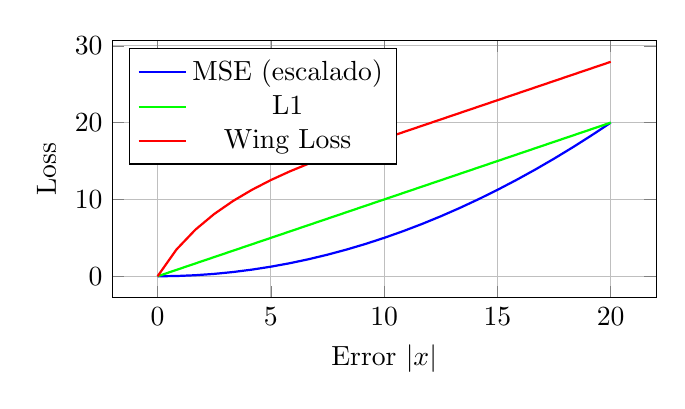
\begin{tikzpicture}
        \begin{axis}[
            xlabel={Error $|x|$},
            ylabel={Loss},
            legend pos=north west,
            grid=major,
            width=0.7\textwidth,
            height=0.4\textwidth,
            domain=0:20
        ]
            % MSE
            \addplot[blue, thick] {x^2/20};
            \addlegendentry{MSE (escalado)}

            % L1
            \addplot[green, thick] {x};
            \addlegendentry{L1}

            % Wing Loss (aproximacion)
            \addplot[red, thick] {x < 10 ? 10*ln(1 + x/2) : x - 10 + 10*ln(1 + 10/2)};
            \addlegendentry{Wing Loss}
        \end{axis}
    \end{tikzpicture}
    \caption{Comparacion de funciones de perdida. Wing Loss proporciona mayor sensibilidad para errores pequenos (region logaritmica) mientras mantiene robustez ante outliers (region lineal).}
    \label{fig:loss_comparison}
\end{figure}

\textbf{Ventajas de Wing Loss}:
\begin{enumerate}
    \item \textbf{Gradiente amplificado para errores pequenos}: La derivada en el origen es mayor que en MSE.
    \item \textbf{Robustez ante outliers}: La parte lineal evita que errores grandes dominen el entrenamiento.
    \item \textbf{Transicion suave}: Continuidad en $|x| = \omega$ evita discontinuidades en el gradiente.
\end{enumerate}

Para coordenadas normalizadas en $[0, 1]$, los parametros deben escalarse:

\begin{equation}
    \omega' = \frac{\omega}{S}, \quad \epsilon' = \frac{\epsilon}{S}
    \label{eq:wing_normalized}
\end{equation}

donde $S$ es el tamano de la imagen (224 en este trabajo).

\subsection{Adaptive Wing Loss}

\textbf{Adaptive Wing Loss} \cite{wang2019adaptive} extiende Wing Loss adaptando los parametros segun la dificultad de cada landmark:

\begin{equation}
    \mathcal{L}_{\text{AWL}}(y) = \begin{cases}
        \omega \ln(1 + |y/\epsilon|^{\alpha - y}) & \text{si } |y| < \theta \\
        A|y| - C & \text{en otro caso}
    \end{cases}
    \label{eq:adaptive_wing}
\end{equation}

donde $\alpha$ controla la forma de la curva y $\theta$ es el umbral adaptativo.

% -----------------------------------------------------------------------------
\section{Tecnicas de Regularizacion}
\label{sec:regularizacion}
% -----------------------------------------------------------------------------

La regularizacion previene el sobreajuste (overfitting) y mejora la generalizacion del modelo.

\subsection{Dropout}

\textbf{Dropout} \cite{srivastava2014dropout} desactiva aleatoriamente una fraccion $p$ de las neuronas durante el entrenamiento:

\begin{equation}
    \vec{h}_{\text{drop}} = \vec{m} \odot \vec{h}, \quad m_i \sim \text{Bernoulli}(1-p)
    \label{eq:dropout}
\end{equation}

donde $\odot$ denota el producto elemento a elemento.

Durante la inferencia, las activaciones se escalan por $(1-p)$ para mantener la misma esperanza. En este trabajo se utiliza $p = 0.3$, valor determinado experimentalmente como optimo.

\subsection{Normalizacion por Lotes y Grupos}

\textbf{Batch Normalization} \cite{ioffe2015batch} normaliza las activaciones usando estadisticas del mini-batch:

\begin{equation}
    \hat{x}_i = \frac{x_i - \mu_B}{\sqrt{\sigma_B^2 + \epsilon}}
    \label{eq:batchnorm}
\end{equation}

donde $\mu_B$ y $\sigma_B^2$ son la media y varianza del batch.

\textbf{Group Normalization} \cite{wu2018group} agrupa los canales y normaliza dentro de cada grupo:

\begin{equation}
    \hat{x}_i = \frac{x_i - \mu_G}{\sqrt{\sigma_G^2 + \epsilon}}
    \label{eq:groupnorm}
\end{equation}

\begin{nota}
En este trabajo se utiliza GroupNorm en lugar de BatchNorm en la cabeza de regresion porque:
\begin{itemize}
    \item Es independiente del tamano del batch
    \item Mas estable con batch sizes pequenos (8 en fine-tuning)
    \item Mejor rendimiento experimental en este problema
\end{itemize}
\end{nota}

\subsection{Data Augmentation}
\label{subsec:data_augmentation}

La \textbf{aumentacion de datos} genera variaciones de las muestras de entrenamiento, incrementando efectivamente el tamano del dataset:

\begin{itemize}
    \item \textbf{Flip horizontal}: Reflexion especular con intercambio de landmarks simetricos
    \item \textbf{Rotacion}: Rotacion aleatoria de $\pm 10\degree$
    \item \textbf{Jitter de color}: Variaciones de brillo ($\pm 20\%$) y contraste ($\pm 20\%$)
\end{itemize}

\begin{algorithm}[H]
\caption{Flip Horizontal con Intercambio de Landmarks}
\label{alg:flip}
\begin{algorithmic}[1]
    \Require Imagen $I$, landmarks $L \in \R^{15 \times 2}$, pares simetricos $P$
    \Ensure Imagen y landmarks transformados
    \State $I' \leftarrow \text{flip}(I, \text{axis}=\text{horizontal})$
    \State $L'[:, 0] \leftarrow 1 - L[:, 0]$ \Comment{Invertir coordenada X}
    \For{$(i, j) \in P$} \Comment{$P = \{(2,3), (4,5), (6,7), (11,12), (13,14)\}$}
        \State $L'[i], L'[j] \leftarrow L'[j], L'[i]$ \Comment{Intercambiar pares}
    \EndFor
    \State \Return $I'$, $L'$
\end{algorithmic}
\end{algorithm}

% -----------------------------------------------------------------------------
\section{Preprocesamiento de Imagenes Medicas}
\label{sec:preprocesamiento}
% -----------------------------------------------------------------------------

\subsection{CLAHE}
\label{subsec:clahe}

\textbf{CLAHE} (Contrast Limited Adaptive Histogram Equalization) \cite{pizer1987adaptive} es una tecnica de mejora de contraste local que divide la imagen en regiones (tiles) y ecualiza el histograma de cada region independientemente.

\begin{definicion}[CLAHE]
Para cada tile de la imagen:
\begin{enumerate}
    \item Calcular el histograma local
    \item Limitar (clip) los picos del histograma al valor \textit{clip\_limit}
    \item Redistribuir los pixeles recortados uniformemente
    \item Ecualizar el histograma resultante
    \item Interpolar bilinealmente en los bordes de tiles adyacentes
\end{enumerate}
\end{definicion}

Los parametros clave son:
\begin{itemize}
    \item \textbf{clip\_limit}: Controla el contraste maximo (valores tipicos: 1.0-4.0)
    \item \textbf{tile\_size}: Tamano de la cuadricula (valores tipicos: 4-16)
\end{itemize}

\begin{figure}[htbp]
    \centering
    \includegraphics[width=0.9\textwidth]{clahe_comparison.png}
    \caption{Efecto de CLAHE en radiografias de las tres categorias. CLAHE realza los bordes anatomicos, especialmente en zonas con consolidaciones pulmonares (COVID-19).}
    \label{fig:clahe_effect}
\end{figure}

En este trabajo se encontro que \texttt{clip\_limit=2.0} y \texttt{tile\_size=4} proporcionan el mejor balance para radiografias toracicas, particularmente efectivo para casos de COVID-19 donde las consolidaciones oscurecen los bordes pulmonares.

\subsection{Normalizacion ImageNet}

Las imagenes se normalizan usando las estadisticas de ImageNet para compatibilidad con los pesos preentrenados:

\begin{equation}
    \hat{I} = \frac{I - \vec{\mu}}{\vec{\sigma}}
    \label{eq:imagenet_norm}
\end{equation}

donde $\vec{\mu} = [0.485, 0.456, 0.406]$ y $\vec{\sigma} = [0.229, 0.224, 0.225]$.

% -----------------------------------------------------------------------------
\section{Ensemble Learning}
\label{sec:ensemble}
% -----------------------------------------------------------------------------

El \textbf{aprendizaje por ensemble} combina predicciones de multiples modelos para mejorar el rendimiento y reducir la varianza.

\subsection{Motivacion Teorica}

Sea $\hat{y}_i$ la prediccion del modelo $i$ con error $\epsilon_i$:

\begin{equation}
    \hat{y}_i = y + \epsilon_i
    \label{eq:model_error}
\end{equation}

Si los errores son independientes con media cero y varianza $\sigma^2$, el promedio de $M$ modelos tiene varianza:

\begin{equation}
    \text{Var}\left(\frac{1}{M}\sum_{i=1}^{M} \hat{y}_i\right) = \frac{\sigma^2}{M}
    \label{eq:ensemble_variance}
\end{equation}

En la practica, los errores no son completamente independientes, pero el ensemble aun reduce la varianza significativamente.

\subsection{Estrategias de Ensemble}

\begin{enumerate}
    \item \textbf{Promedio simple}: Todas las predicciones tienen peso igual
    \begin{equation}
        \hat{y}_{\text{ens}} = \frac{1}{M}\sum_{i=1}^{M} \hat{y}_i
        \label{eq:simple_avg}
    \end{equation}

    \item \textbf{Promedio ponderado}: Pesos basados en rendimiento individual
    \begin{equation}
        \hat{y}_{\text{ens}} = \sum_{i=1}^{M} w_i \hat{y}_i, \quad \sum_{i} w_i = 1
        \label{eq:weighted_avg}
    \end{equation}
\end{enumerate}

\begin{nota}
Experimentalmente se encontro que el promedio simple es tan efectivo como esquemas de ponderacion mas complejos para este problema, siempre que se excluyan modelos de rendimiento significativamente inferior.
\end{nota}

% -----------------------------------------------------------------------------
\section{Test-Time Augmentation}
\label{sec:tta}
% -----------------------------------------------------------------------------

\textbf{Test-Time Augmentation} (\TTA) aplica transformaciones durante la inferencia y promedia las predicciones, reduciendo la varianza sin reentrenar:

\begin{algorithm}[H]
\caption{Test-Time Augmentation para Landmarks}
\label{alg:tta}
\begin{algorithmic}[1]
    \Require Imagen $I$, modelo $f$
    \Ensure Prediccion promediada $\hat{L}$
    \State $\hat{L}_1 \leftarrow f(I)$ \Comment{Prediccion original}
    \State $I_{\text{flip}} \leftarrow \text{flip}(I)$
    \State $\hat{L}_2 \leftarrow f(I_{\text{flip}})$
    \State $\hat{L}_2 \leftarrow \text{inverse\_flip}(\hat{L}_2)$ \Comment{Corregir coordenadas e intercambiar pares}
    \State $\hat{L} \leftarrow (\hat{L}_1 + \hat{L}_2) / 2$
    \State \Return $\hat{L}$
\end{algorithmic}
\end{algorithm}

En este trabajo, \TTA proporciona una mejora consistente de 0.3-0.5 pixeles sin costo de entrenamiento adicional.

% -----------------------------------------------------------------------------
\section{Metricas de Evaluacion}
\label{sec:metricas}
% -----------------------------------------------------------------------------

\subsection{Error Euclidiano}

La metrica principal para deteccion de landmarks es el error euclidiano (distancia) entre prediccion y ground truth:

\begin{equation}
    e_i = \|\hat{\vec{p}}_i - \vec{p}_i\|_2 = \sqrt{(\hat{x}_i - x_i)^2 + (\hat{y}_i - y_i)^2}
    \label{eq:euclidean_error}
\end{equation}

\subsection{Metricas Agregadas}

\begin{itemize}
    \item \textbf{Error medio}: $\bar{e} = \frac{1}{N}\sum_{i=1}^{N} e_i$
    \item \textbf{Desviacion estandar}: $\sigma_e = \sqrt{\frac{1}{N}\sum_{i=1}^{N}(e_i - \bar{e})^2}$
    \item \textbf{Mediana}: Valor central ordenado, mas robusta ante outliers
    \item \textbf{Percentiles}: $P_{90}$, $P_{95}$ para caracterizar la cola de la distribucion
\end{itemize}

\subsection{Success Rate}

El \textit{success rate} mide el porcentaje de predicciones bajo un umbral dado:

\begin{equation}
    \text{SR}(\tau) = \frac{1}{N} \sum_{i=1}^{N} \mathbb{1}[e_i < \tau]
    \label{eq:success_rate}
\end{equation}

% -----------------------------------------------------------------------------
% FIN DEL CAPITULO
% -----------------------------------------------------------------------------
